\setAuthor{Tundmatu autor}
\setRound{lahtine}
\setYear{2007}
\setNumber{G 6}
\setDifficulty{3}
\setTopic{Dünaamika}

\prob{Karatist}
Hinnake, millise kiirusega $v$ peab karatisti käsi tabama kahele kivile toetuva lauajupi keskpunkti (vt joonist), et laud murduks? Käe mass on $m = \SI{1,5}{kg}$, laua mass $M = \SI{2}{kg}$, laua jäikustegur $k = \SI{1,4e5}{N/m}$, murdumiseks vajalik läbipaine (st laua keskpunkti nihe) $d = \SI{20}{mm}$. 

\emph{Märkus}. Jäikustegur $k$ on võrdetegur laua keskpunkti rakendatud jõu $F$ ning laua keskpunkti nihke $x$ vahel (vt joonist).

\begin{center}
	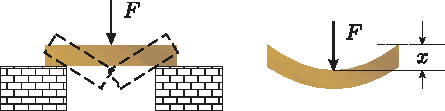
\includegraphics[width=0.8\linewidth]{2007-lahg-06-yl}
\end{center}

\hint
Löögi hetkel kehtib impulsi jäävus, aga energia ei säili. See-eest säilib mehaaniline energia pärast põrget toimuval liikumisel.

\solu
Laua paindumist käsitleme sarnaselt vedru paindumisega. Laua elastsusenergia enne purunemist on $E = kx^2/2$. Eeldame, et pärast plastset põrget toimuval liikumisel on mehaaniline energia jääv ning lauajupp ja käsi peatuvad vahetult pärast lööki. Käe ja laua kokkupõrge --- löök --- on täielikult mitteelastne. Seega peab pärast lööki laua ja rusika kineetilisest energiast
\[
W = \frac{(m+M)u^2}{2}
\]
piisama laua deformeerimiseks.
\[
E=W \quad \Rightarrow \quad u=\sqrt{\frac{k d^{2}}{m+M}},
\]
kus $u$ on laua ja käe kiirus pärast lööki. Löögi hetkel kehtib impulsi jäävus
\[
(m+M) u=m v \quad \Rightarrow \quad v=\frac{m+M}{m} u.
\]
Kokkuvõttes saame
\[
	v=\frac{m+M}{m} \sqrt{\frac{k d^{2}}{m+M}}=\sqrt{\frac{k d^{2}(m+M)}{m^{2}}},
\]
\[
	 v=\sqrt{\frac{\num{1,4} \cdot 10^{5} \cdot \num{0,02}^{2} \cdot(\num{1,5}+2)}{\num{1,5}^{2}}} \approx \SI{9,3}{m/s}.
\]
\probend